\documentclass{article}
\usepackage{amsfonts}
\usepackage[colorlinks=true,citecolor=blue,urlcolor=cyan,linkcolor=red]{hyperref}
\usepackage{amssymb}
\usepackage{amsmath,amssymb,amscd,epsfig,amsfonts,rotating}
\usepackage{graphicx}
\usepackage{epsfig}
\usepackage{multirow}
\usepackage{booktabs}
\usepackage{url}
\usepackage[margin=1.5in]{geometry}

\newtheorem{def:def}{Definition}
\newtheorem{thm:thm}{Theorem}
\newtheorem{thm:lm}{Lemma}

\DeclareMathOperator*{\argmax}{arg \, max}
\DeclareMathOperator*{\var}{var}
\DeclareMathOperator*{\cov}{cov}
\newcommand{\bs}{\boldsymbol}

\title{Variational Auto-Encoder for Text Representation Learning \\\Large{CS410 Tech Review}}
\author{Jinning Li\\
{\small University of Illinois at Urbana-Champaign}\\
{\small jinning4@illinois.edu}}
\date{}
\begin{document}
\maketitle

\section{Introduction}
The deep neural networks have inspired a large progress on the text related tasks. There are many interesting computational textual tasks such as text classification, text translation, and text generation. During most of these tasks, one important question is how to extract the vector representation from a piece of text so that the text will become easier to be processed. The text representation learning is to map the text to a vector space with a relatively low dimension. During this process, the property of the text should be kept. For example, the similarity between two pieces of text can be calculated by the cosine distance between two vectors in this vector space.

Variational Autoencoder (VAE) is a deep learning technique for learning the latent representations. And the autoencoder is a kind of neural network which is designed to learn an indentity function in an unsupervised way to reconstruct the original input signal. In this process, the data is compressed so that a more efficient and compressed representation is learned~\cite{hinton2006reducing}. The autoencoder contains two parts: the encoder network and the decoder network. The encoder network translates the original high-dimensional input into a low-dimensional one. The decoder recovers the low-dimensional signal to the original one. After we train the autoencoder, we can use the encoder to do the dimension reduction. We can also make use of the decoder network to generate samples.

Developing VAE for text representation learning is always a interesting and challenge works. In computer vision tasks, the inputs are images with the forms of pixels, which is easier for the computer to process, especially after the convolutional neural networks become popular. However, the text format is harder for the computer to understand. There may be problems of ambiguity. In this survey, we will introduce the state-of-the-art VAE techniques to learn text representations.

\section{Variational Auto-Encoder}
The autoencoder is a popular neural network designed to accomplish the dimension reduction. Similar method include pricipal component analysis (PCA) and Matrix Factorization (MF).
\begin{figure}[ht]
%   	\vspace{-mm}
  \centering
  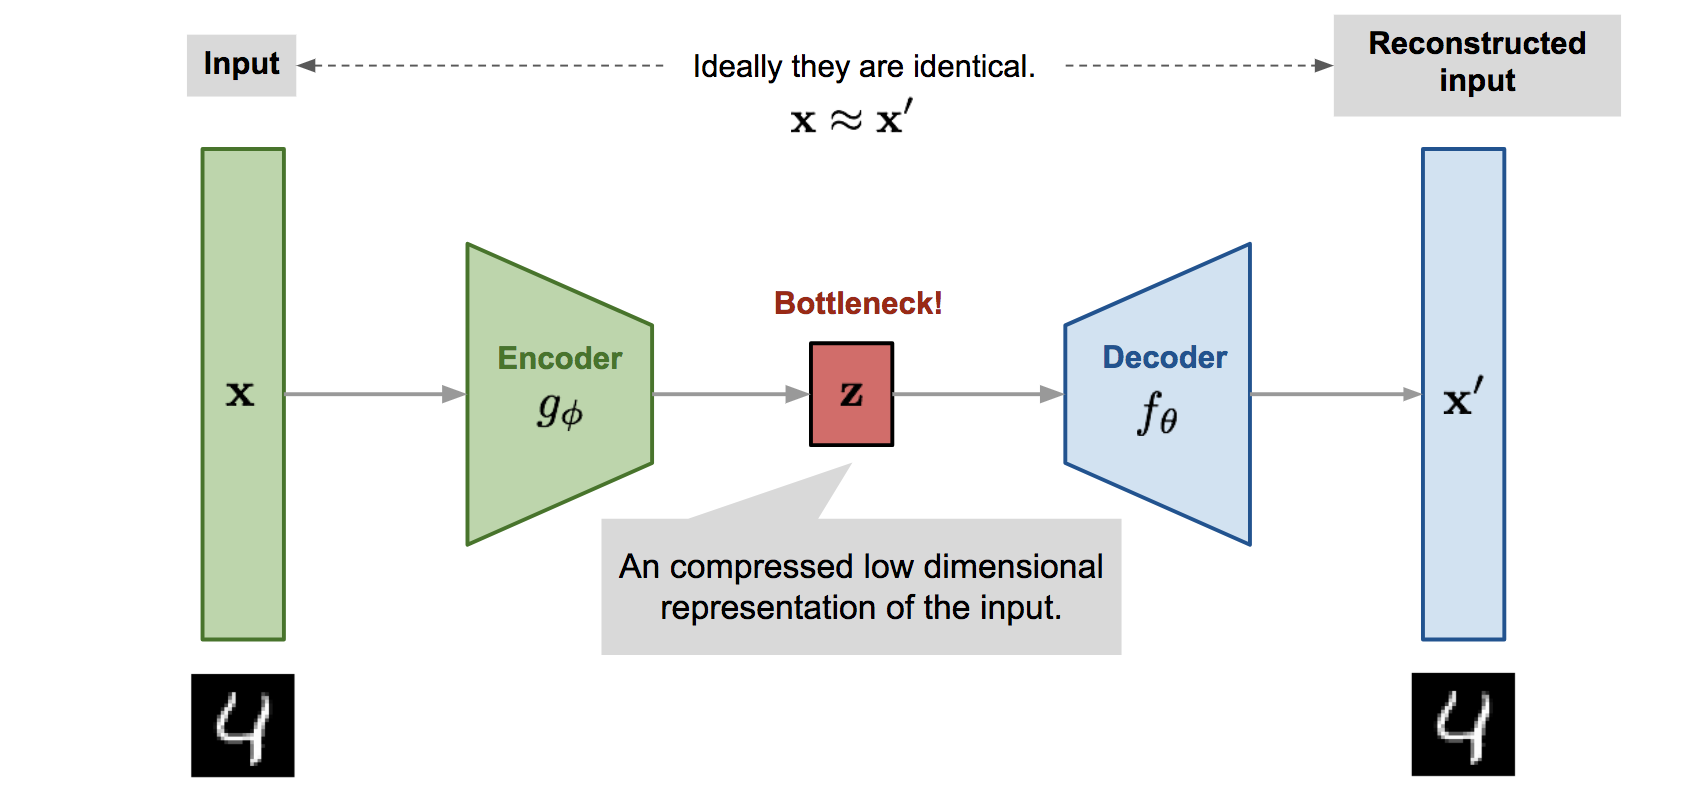
\includegraphics[width = 0.8\linewidth]{figures/autoencoder-architecture.png}
  %	\vspace{-9mm}
  \caption{The architecture of autoencoder model~\cite{weng2018VAE}}
  \label{fig::fig}
  % \vspace{-8pt}
\end{figure}
The architecture of autoencoder contains an encoder mapping function $g(\cdot)$ with parameters $\phi$ and a decoder function $f(\cdot)$ with parameters $\theta$. The autoencoder will learn a low-dimensional latent vector $z=g_{\phi}(x)$ from the input $x$. The reconstruct input is $x'=f_{\theta}(g_{\phi}(x))$. The parameters are trained to make the reconstructed signal $x'$ similar to the original input $x$, which is $x'=f_{\theta}(g_{\phi}(x))\rightarrow x$. Practically, this can be achieved by optimize an object such as minizing a MSE loss:
\begin{equation}
L(\theta, \phi) = \frac{1}{n}\sum_{i=1}^{n}(x_i-f_\theta(g_\phi(x_i)))^2
\end{equation}

The Variational Autoencoder (VAE) is similar to the autoencoder. However, VAE does not map the input into a fixed vector. VAE will map the the input into a distribution.

\begin{figure}[ht]
%   	\vspace{-mm}
  \centering
  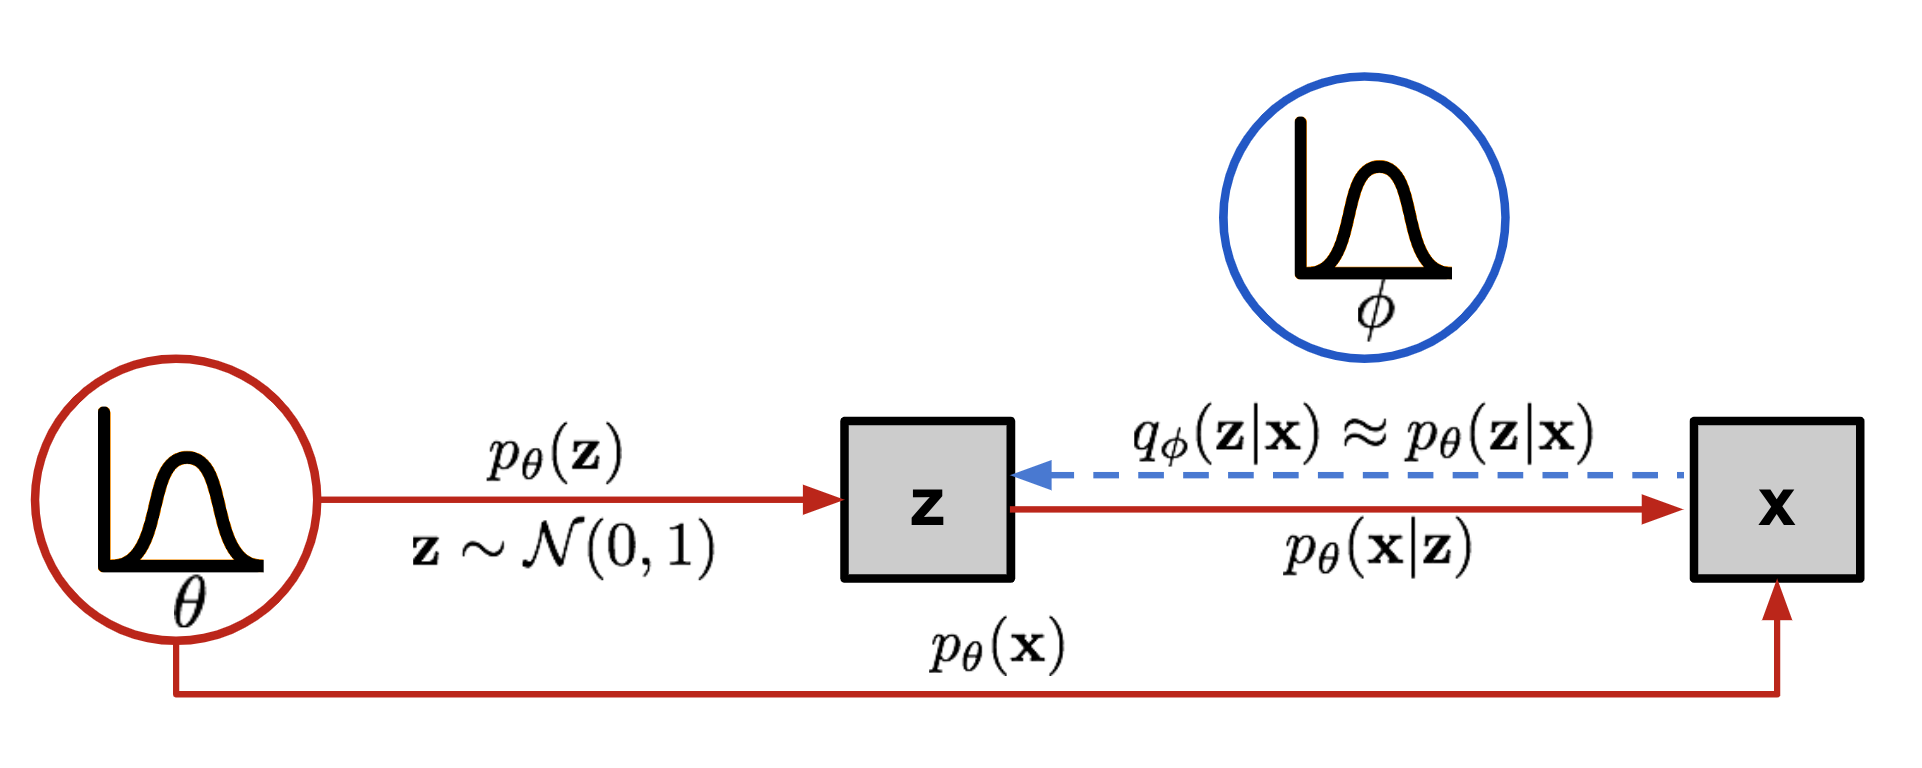
\includegraphics[width = 0.7\linewidth]{figures/VAE-graphical-model.png}
  %	\vspace{-9mm}
  \caption{The graphical model involved in Variational Autoencoder}
  \label{fig::VAE}
  % \vspace{-8pt}
\end{figure}

\section{Variational Auto-Encoder for Text Representation Learning}
The Variational Auto-Encoder (VAE) has been widely used in computer vision tasks, such as image generating and style transfer. Beta-VAE~\cite{higgins2016beta} is a good example. Higgins et al. (2016) proposes this method, which is a modification of VAE to discover disentangled latent factors. The disentanglement means every variable in the latent representation is sensitive to one single generative factor and invariant to other factors. This disentangled feature is critical for the interpretability of neural network. For example, the skin color, hair color, glasses of an image of persons. The Beta-VAE technique maximizes the probability to generate the real data and keeps the distance between the real and estimated distribution small enough. The loss Function of Beta-VAE is:
\begin{equation}
	L=-\textsc{E}_{z\sim q_{\phi}}(z|x)\log p_{\theta}(x|z) + \beta D_{KL}(q_\phi(z|x)\|p_\theta(z))
\end{equation}

\begin{figure}[ht]
%   	\vspace{-mm}
  \centering
  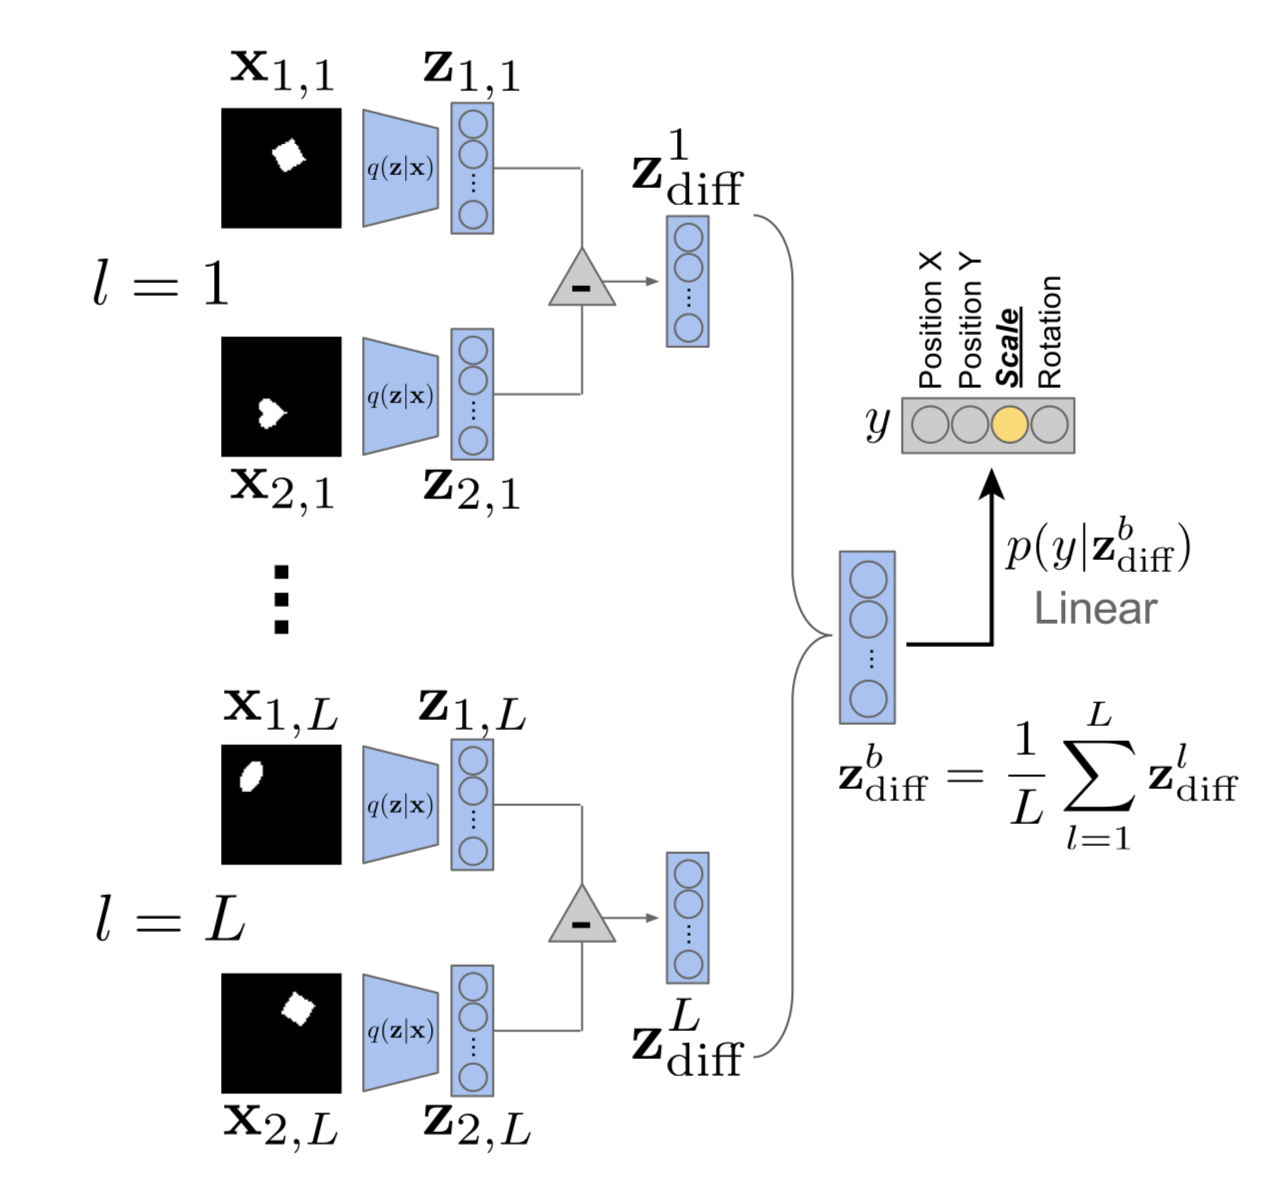
\includegraphics[width = 0.56\linewidth]{figures/betavae.png}
  %	\vspace{-9mm}
  \caption{The disentanglement metric of Beta-VAE}
  \label{fig::Beta-VAE}
  % \vspace{-8pt}
\end{figure}

VAE is also widely used in the text representation learning. Guo et al. (2020)~\cite{10.1007/978-3-030-60029-7_21} proposes a CNN-VAE model for text representation learning. In this paper, the author combine the network framework of the VAE and the convolutional neural networks (CNN) to extract the text feature representation and applt it to the text classification task. In this work, CNN is used to realize the network structure of VAE since CNN can learn better local features from the input signal. CNN is applied in the framework of VAE, therefore the vector feature space conform to the Gaussian didistrubution.

\begin{figure}[ht]
%   	\vspace{-mm}
  \centering
  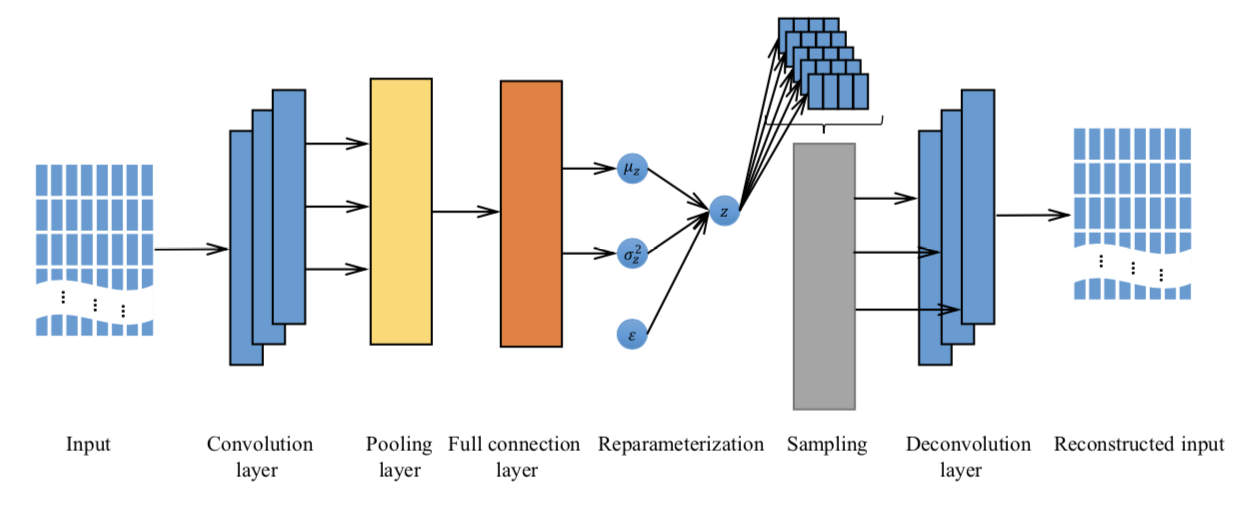
\includegraphics[width = 0.75\linewidth]{figures/cnnvae.png}
  %	\vspace{-9mm}
  \caption{The structure of CNN-VAE}
  \label{fig::CNN-VAE}
  % \vspace{-8pt}
\end{figure}

The interpretability of VAE is also a popular topic for the researchers. John et al.~\cite{john2018disentangled} proposes a simple but efficient approach. The model is trained with a incorporated objective of auxiliary multi-task and adversarial objectives. They result of this method shows that the style and content are indeed disentangled in the latent space. This disentangled latent representation learning method is applied to style transfer on non-parallel corpora.

\begin{figure}[ht]
%   	\vspace{-mm}
  \centering
  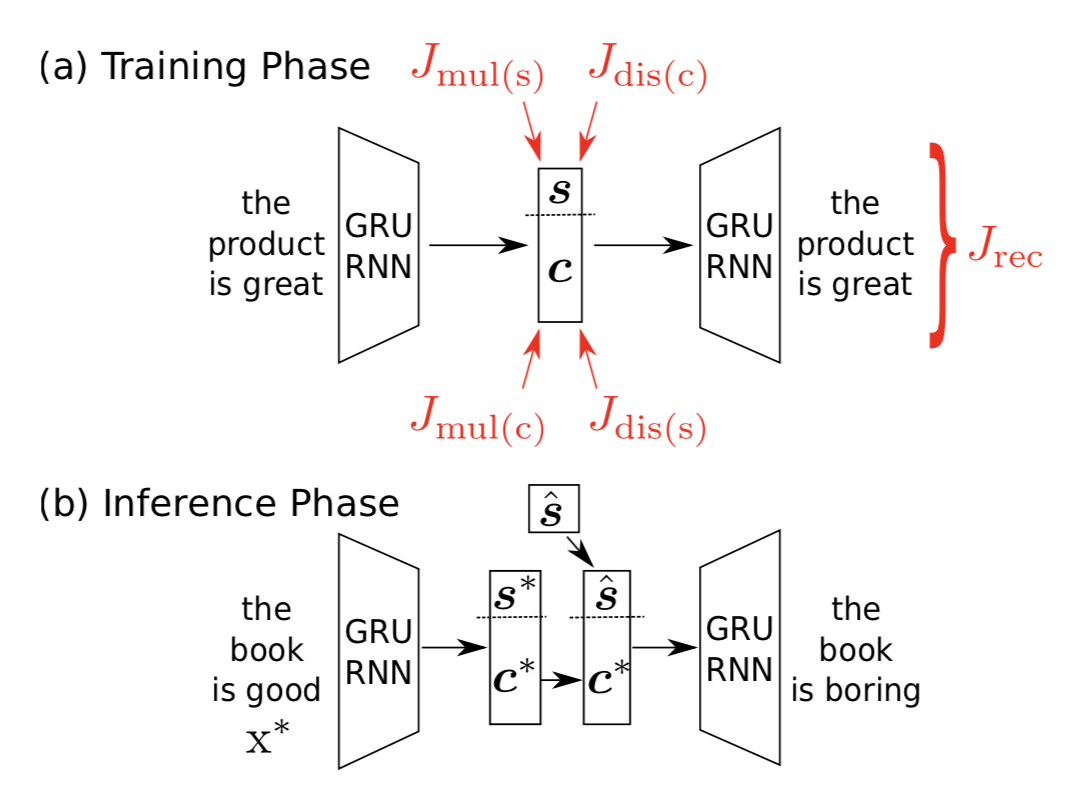
\includegraphics[width = 0.6\linewidth]{figures/john.png}
  %	\vspace{-9mm}
  \caption{The structure of John et al. (2018)}
  \label{fig::CNN-VAE}
  % \vspace{-8pt}
\end{figure}

\section{conlusion}
The variational auto-encoder (VAE) has been proved to be effective on the computer vision tasks and there are also many existing works to apply VAE on the textual tasks. One of the challenge of the textual scenario is the interpretability because the text is not that obvious for congnition as the image. Some existing works such as John et al. (2018)'s work has tried to develop new mult-task objective to make the learnt text representation disentangled. The possible future work can be improving the quality of latent representation with other additional knowledge basis.

\bibliographystyle{abbrv}
\bibliography{techreview}


\end{document}
